\documentclass[12pt, a4paper]{article}
\usepackage[utf8]{inputenc}
\usepackage[margin=2.5cm]{geometry}

\usepackage{amssymb,amsmath}
\usepackage{enumerate}
\usepackage[dvipsnames]{xcolor}
\usepackage{graphicx}
\usepackage{caption}
\usepackage{sfmath}
\usepackage{changepage}
\usepackage{hyperref}
\usepackage{ragged2e}
\usepackage{parskip}
\usepackage[english]{babel}
\usepackage{seqsplit}
\usepackage{bm}

\renewcommand{\familydefault}{\sfdefault}
\usepackage[lighttt]{lmodern}

\newcommand{\hlinesep}{\noindent \rule{\textwidth}{0.5pt}\vspace{6pt}}

\usepackage{newfloat}
\usepackage{minted}
\setminted{
bgcolor = gray!20,
breaklines,
python3
}
\newcommand{\inlinecode}[1]{\mintinline[breaklines, bgcolor=gray!20, python3]{python}{#1}}

\renewcommand{\figurename}{Fig.}

\newcommand{\code}[1]{\colorbox{gray!25}{\texttt{#1}}}

\newcommand{\filestamp}[1]{\underline{\textbf{file: #1}}}
\newcommand{\red}[1]{\textcolor{red}{#1}}
\newcommand{\matrixel}[3]{\left\langle{#1}\middle|{#2}\middle|{#3}\right\rangle}
\newcommand{\trace}[1]{\mathrm{tr}\left({#1}\right)}
\newcommand{\ket}[1]{\left|{#1}\right\rangle}
\newcommand{\bra}[1]{\left\langle{#1}\right|}
\newcommand{\expval}[1]{\left\langle{#1}\right\rangle}
\newcommand{\comm}[2]{\left[{#1},{#2}\right]}
\newcommand{\acomm}[2]{\left\{{#1},{#2}\right\}}
\newcommand{\imag}[1]{\mathrm{Im}\left\{{#1}\right\}}
\newcommand{\real}[1]{\mathrm{Re}\left\{{#1}\right\}}
\newcommand{\dissip}[1]{\mathcal{D}\left({#1}\right)\left[\rho\right]}
\newcommand{\smalleq}[2][0.75]{\text{\scalebox{#1}{$#2$}}}
\newcommand{\bop}{\hat{b}}
\newcommand{\bopn}[1]{\bop^{#1}}
\newcommand{\bdag}{\bop^\dagger}
\newcommand{\bdagn}[1]{\bop^{\dagger {#1}}}
\newcommand{\bmbn}[2]{\bdagn{#1}\bop^{#2}}

\newcommand{\pybolano}{\texttt{pyBoLaNO}~}

\newenvironment{revision}{%
\color{red}
}
{}

%%%%%%%%%%%%%%%%%%%%%%%%%%%%%%%%%%%%%%%%%

\newcommand{\review}[1]{
\newpage
\phantomsection
\vspace*{\fill}
\begin{center}
\Large{\uppercase{{\textbf{Reply to Report of Reviewer {#1}}}}}
\end{center}
\vspace*{\fill}
}

%%%%%%%%%%%%%%%%%%%%%%%%%%%%%%%%%%%%%%%%%

\newcommand{\addendum}{
\newpage
\phantomsection
\vspace*{\fill}
\begin{center}
\Large{\uppercase{\textbf{Addendum}}}
\end{center}
\vspace*{\fill}
\newpage
}

%%%%%%%%%%%%%%%%%%%%%%%%%%%%%%%%%%%%%%%%%

\newenvironment{revremark}{%
\newpage
\phantomsection
\color{RoyalPurple}
\par
\textbf{REVIEWER'S REMARK:}
\par
}
{}

%%%%%%%%%%%%%%%%%%%%%%%%%%%%%%%%%%%%%%%%%

\newenvironment{revthanks}{%
\color{Black}
\textbf{AUTHORS:}
\par 
We thank you for reviewing our manuscript and providing insightful responses. Below are our responses to your questions/comments.
}
{}

%%%%%%%%%%%%%%%%%%%%%%%%%%%%%%%%%%%%%%%%%

\newenvironment{revq}[1]{%
\newpage\phantomsection
\color{RoyalPurple}
\par
\textbf{QUESTION/COMMENT {#1}:}
\par
}
{\bigskip}

%%%%%%%%%%%%%%%%%%%%%%%%%%%%%%%%%%%%%%%%%

\newenvironment{reva}{%
\color{Black}
\par
\textbf{REPLY:}
\par
}
{\bigskip}

%%%%%%%%%%%%%%%%%%%%%%%%%%%%%%%%%%%%%%%%%

\newenvironment{revpre}{%
\textbf{{BEFORE REVISION:}}
\par
}
{\bigskip}

%%%%%%%%%%%%%%%%%%%%%%%%%%%%%%%%%%%%%%%%%

\newenvironment{revpost}{%
\textbf{{AFTER REVISION:}}
\par
}
{}

%%%%%%%%%%%%%%%%%%%%%%%%%%%%%%%%%%%%%%%%%

\setlength{\parindent}{0pt}

\usepackage{setspace}
\onehalfspacing

%---------------------------------------------------
\begin{document}

\sloppy

\pagenumbering{gobble}

\begin{flushright}
    South Tangerang, \today
\end{flushright}

\bigskip

Dear Editor of Computer Physics Communications (CPC), 

Thank you for sending us the referee reports and the invitation to submit a revised version of our article titled ``pyBoLaNO: A Python symbolic package for normal ordering involving bosonic ladder operators'' (COMPHY-D-25-00012).

We have carefully read the reports of the two reviewers and thank them for kindly evaluating the manuscript.

We fully address all the comments and questions from the reviewers by revising some parts of the manuscript, as well as the source code of our package. The revised parts of the manuscript are indicated in \textcolor{red}{red} in the compiled PDF file, while in the LaTeX source we use a self-defined environment \verb|\begin{revision}...\end{revision}|, which can be safely deleted by the copy-editor once this manuscript can go to the production stage.

Enclosed with this response letter, we provide more detailed answers to each comment/question, alongside the corresponding changes made to the manuscript. We have also included some addenda to the manuscript upon checking our manuscript and finding some errors. We describe the changes after we address the reviewer's reports in this message. 

We thank you for your consideration and look forward to hearing from you.

\bigskip
\hrule
\bigskip

Corresponding author:

\textbf{Hendry Minfui Lim}\

\url{hendry01@ui.ac.id}

{Research Center for Quantum Physics, National Research and Innovation Agency (BRIN), South Tangerang 15314, Indonesia}

{Department of Physics, Faculty of Mathematics and Natural Sciences, Universitas Indonesia, Depok 16424, Indonesia}

%%%%%%%%%%%%%%%%%%%%%%%%%%%%%%%%%%%%%%%%%%%%%%%%%%%%%%%%%%%%%%%%%%%%%%%%%%%%%%%%

\review{1}

%%%

\begin{revremark}
We have attached a file with feedback.
\end{revremark}

\begin{revthanks}Unfortunately, the attached file seems to be missing from the review report sent to us. Since we received this report, we have mailed the Editor to obtain the file but have yet to receive any response upon completing this round of revision. As such, we are unable to address the feedback given in the file. Nevertheless, at this moment we can at least respond to your other comments present in the report. If you are not satisfied with our answers, we are happy to continue to the next revision stage.
\end{revthanks}

%%%

\begin{revq}{1}
It appears that some (or all) of the functionality is available elsewhere
(https://github.com/sympy/sympy/tree/master/sympy/physics/quantum/operatorordering.py).
\end{revq}

\begin{reva}
We thank the reviewer for pointing this out. We admit that we are unaware of \code{sympy.physics.} \code{quantum.operatorordering}, as probably evident from the commit history of our GitHub repository. Our package, formerly named \code{boson\_ladder}, used the same algorithm as that in \texttt{SymPy}, where the commutation relations are recursively used to reorder the operators (see, for example, \href{https://github.com/hendry24/pyBoLaNO/commit/a234f48a53158e1c9502d17959dfb6a72fcde767}{\texttt{Commit a234f48}}, which is before the addition of Blasiak's formulae). Then, we found one critical drawback to this method: \emph{the resulting recursion tree is highly inefficient}. 

Similar to normal-ordering by hand, the method currently applied in \texttt{SymPy} grows quickly in computation cost as the number of ladder operators increases and the excess (the difference between the number of annihilation operators and creation operators in the expression) decreases. For example, the normal ordering of $\hat{b}^{10}\hat{b}^{\dagger 10}$ takes more than $10$ seconds on the corresponding author's personal computer. This limitation is overcome by Blasiak's formulae, which provide an explicit formula for the normal-ordered equivalent of any given expression involving the ladder operators. 

We further realized that the claim that normal ordering functionalities are absent in \texttt{SymPy} \code{ver.1.13.3} was also incorrect. \textbf{However}, we believe that the \textbf{more efficient method implemented in our package}, as well as the \textbf{convenient way for computing the evolution of any expectation value} within the Lindblad master equation framework, can serve as \textbf{novelties worth publishing}. 

To address this comment, we have made several significant changes to the manuscript:
\begin{enumerate}
    \item We deleted our incorrect claim and reworded our motivation for writing the package, highlighting its novelties over the conventional \texttt{SymPy}. 
    \item We have added a benchmark against \texttt{SymPy}'s implementation in Section 5 (Performance) to demonstrate the superiority of the explicit formulae.
    \item As we are uncertain of how SymPy's developers will resolve this conflict (were it be one), we have decided to not use the ladder operator objects in SymPy and instead wrote our package's own base for the ladder operator object, \texttt{pybolano.utils.operators.pybolanoOp}, which are similar to \texttt{sympy.physics.secondquant.SqOperator} in construction. It is added with \href{https://github.com/hendry24/pyBoLaNO/commit/8838d27293e6475f92c1827ddb7ad3e6f3e8471a}{\texttt{Commit 8838d27}}.
\end{enumerate}
\end{reva}

\newpage

\begin{revpre}

\textbf{(paragraphs 2--3 of Section 1 of the original manuscript)}

As the system description becomes more complex, the algebraic manipulation of the dynamical equations becomes more tedious and prone to errors. As such, a calculator that does the algebra is desirable. The \texttt{SymPy} package~\cite{meurer_sympy_2017} provides a symbolic computation framework in the \texttt{Python} programming language. At the time of writing this work, \texttt{SymPy} is on release \inlinecode{ver. 1.13.3}, which supports the ladder operators via the \inlinecode{sympy.physics.secondquant} submodule. However, the support is limited to arithmetic operations. The function \inlinecode{wicks} for normal (Wick) ordering is not implemented for bosonic ladder operators. In practice, we often desire to evaluate the normal ordering of operators involving bosonic ladder operators. An example of such cases, which motivates us for this work, is the evolution of the expectation values for open quantum systems described by the Lindblad master equation~\cite{schlosshauer_decoherence_2007, breuer_theory_2002}. If analytical expressions are not the concern, several packages are available to solve the problem numerically, e.g., \texttt{QuTiP}~\cite{johansson_qutip_2012, johansson_qutip_2013} and \texttt{QuantumOptics.jl}~\cite{Kramer2018}. Otherwise, to our knowledge~\cite{chia_relaxation_2020, Shen2023, downing_hyperbolic_2024, Krimer2019, Zens2019, Ahmadi2024, Downing2021, Downing2022, Downing2023, BenArosh2021, Amitai2018.PhysRevE.97.052203, Minganti2019, Chimczak2023, Farina2019, Zhang2021}, there is yet a symbolic computational package that facilitates the solution to the problem.

In this work, we develop the \texttt{Python} package \pybolano that offers fast symbolic normal ordering of expressions involving bosonic ladder operators, which extends to fast normal ordering of commutators and expectation value evolution from the Lindblad master equation.  The package is fully built on and compatible with \texttt{SymPy}. It supports multipartite descriptions and multiprocessing for each additive term in the input(s). 

\textbf{(paragraphs 1 of Section 3.2 of the revised manuscript)}

Instead of calling \inlinecode{AnnihilateBoson(k)} and \inlinecode{CreateBoson(k)} from \inlinecode{sympy.physics.secondquant}, where \inlinecode{k} is the subscript, we recommend using \pybolano's \inlinecode{ops}: 
\begin{minted}[bgcolor=red!15]{python}
ops(k)
\end{minted}
that can be used to construct the annihilation and creation operators. The subscript \inlinecode{k} is optional and can be \inlinecode{Symbol} or any \texttt{Python} object convertible to a string. This function preprocesses \inlinecode{k} into \inlinecode{Symbol}, which is the most compatible with \inlinecode{AnnihilateBoson} and \inlinecode{CreateBoson}. In the current version of \texttt{SymPy}, it also avoids the printing error that occurs when nonzero integers are used as subscripts (which is likely a bug).
\end{revpre}

\newpage

\begin{revpost}

\textbf{(paragraphs 3--4 of Section 1 of the revised manuscript)}

The \texttt{SymPy} package~\cite{meurer_sympy_2017} provides a symbolic computation framework in the \texttt{Python} programming language. \begin{revision}At the time of writing this work, \texttt{SymPy} is on release \inlinecode{ver. 1.13.3} which supports the ladder operators via the \inlinecode{sympy.physics.secondquant} and \inlinecode{sympy.physics.} \inlinecode{quantum} submodules. In particular, normal ordering is implemented as the function \\ \inlinecode{normal_ordered_form}. Unfortunately, the implemented algorithm quickly slows down as we increase the complexity of the expression to normal-order.\end{revision}

\begin{revision}Motivated by a more efficient method and the need for a convenient tool to obtain the expectation value evolution given the equation of motion, we develop the \texttt{Python} package \pybolano that offers fast symbolic normal ordering of expressions involving bosonic ladder operators, which extends to fast normal ordering of commutators and expectation value evolution from the Lindblad master equation. The package is fully built on the core functionalities of \texttt{Sympy} and supports multipartite descriptions as well as multiprocessing for each additive term in the input(s).\end{revision}

\textbf{(paragraphs 1 of Section 3.2 of the revised manuscript)}

\begin{revision}The ladder operator objects are implemented as \inlinecode{BosonicAnnihilationOp} and \inlinecode{BosonicCreationOp}. Instead of initializing both objects, the package provides a convenient call through the function \inlinecode{ops}. By calling\end{revision}
\begin{minted}[bgcolor=red!15]{python}
ops(k)
\end{minted}
we can initialize both annihilation and creation operators with the same subscript. The subscript \inlinecode{k} is optional and can be \inlinecode{Symbol} or any \texttt{Python} object convertible to a string. This function preprocesses \inlinecode{k} into \inlinecode{Symbol} to be used as the subscript of the ladder operators. 
\end{revpost}

%%%

\begin{revq}{2}
We also think the program can only do relatively simple explicit operations, and is less useful in a research setting in which an operator might have a sum over many bosons operators corresponding to different normal modes.
\end{revq}

\begin{reva}
Thank you for your comment. We kindly disagree with this assessment. As pointed out in the manuscript (and in the GitHub \code{README}), our package \textbf{supports the normal ordering of any polynomial containing the ladder operators, including one in a many-body setting}. The algorithm is described in Section 3.3, which we believe is computationally inexpensive considering how the conventional \texttt{SymPy} package works. The computational performance in multipartite settings is discussed in the revised \textbf{Section 5: Performance} and we show how our package is superior to the original \texttt{SymPy}.
\end{reva}

%%%%%%%%%%%%%%%%%%%%%%%%%%%%%%%%%%%%%%%%%%%%%%%%%%%%%%%%%%%%%%%%%%%%%%%%%%%%%%%%%%%%%%%%%%%%%%%%%%%%%%%%%%%%%%%%%%%%%%%%%%%%%

\review{2}

%%%

\begin{revremark}
    In this work, the authors put forth a method for symbolically computing the normal-ordering of Bosonic operators. The authors detail the method behind the work, outline the package organization, and give a set of usage examples. This work is largely based on existing functionality in the SymPy package, and appears to fill a gap in that programs implementation of Wick ordering.
\end{revremark}

\begin{revthanks}
\end{revthanks}

%%%

\begin{revq}{1}
I am curious as to why this is a separate package and not a simple Pull-Request to the SymPy repository? The package does appear to be useful, but I believe the authors should address why their work needs to be a separate installation. 

\end{revq}

\begin{reva}
Thanks for the question. We opted for a separate symbolic package as we prefer a simple package that does specific jobs and desire the freedom to add new relevant features to the package. It is not guaranteed that SymPy will accept every pull request we will be making in the future, as their design philosophy may differ from ours. As an example, \texttt{SymPy} does not natively support multiprocessing, which greatly benefits our normal ordering algorithm. However, we acknowledge the potential value of integration and remain open to collaborating with the \texttt{SymPy} community in the future to explore merging our work if there is sufficient interest. This standpoint is added and described in the second-to-last paragraph of \textbf{Section 1} of the revised manuscript:

---

\begin{revision}Motivated by a more efficient method and the need for a convenient tool to obtain the expectation value evolution given the equation of motion, we develop the \texttt{Python} package \pybolano that offers fast symbolic normal ordering of expressions involving bosonic ladder operators, which extends to fast normal ordering of commutators and expectation value evolution from the Lindblad master equation. The package is fully built on the core functionalities of \texttt{Sympy} and supports multipartite descriptions as well as multiprocessing for each additive term in the input(s).\end{revision}

---

\end{reva}

%%%

\begin{revq}{2}
The authors do not have any unit-tests in their repository. As this package is supposed to be used by other researchers, I would expect some level of testing that gives me confidence in its usage. 
\end{revq}

\begin{reva}
We thank you for your criticism. We have added unit testing to the package you can find at \href{https://github.com/hendry24/pyBoLaNO/tree/main/pybolano/testing}{\texttt{pybolano/testing}}, added with \href{https://github.com/hendry24/pyBoLaNO/commit/8838d27293e6475f92c1827ddb7ad3e6f3e8471a}{\texttt{Commit 8838d27}}.
\end{reva}

%%%

\begin{revq}{3}
The performance section needs to show actual data. In my execution of their code, some cells took $\sim 1$ sec to run, indicating that more complicated examples might take substantially longer. Some kind of scalable example, such as scaling the number of subsystems in a problem, would greatly help in understanding the performance of this work
\end{revq}

\begin{reva}
We thank you for your criticism. While using explicit formulae is arguably the most efficient method, it is indeed good to know for what expressions the evaluation is more computationally costly. We have rewritten Section 5 to discuss the performance of our algorithm in more detail, additionally comparing it to the ``conventional'' method \texttt{SymPy} currently implements. The conclusion has been adjusted accordingly, and we have added a link to the benchmark file in \textbf{Data Availability}.
\end{reva}

\begin{revpre}

\textbf{(Section 5 of the original manuscript)}

Since it is implemented for each summand in the input expression, the speedup gained by using multiprocessing is approximately linear (the evaluation of each summand may take different durations). Meanwhile, the evaluation of a single monomial is optimal because explicit formulae are used.

\textbf{(Section 6 of the original manuscript)}

$\dots$ We have exhibited some examples of use by taking recent results from the literature which also serve to validate the package. We have discussed the computational cost of the normal ordering algorithm. $\dots$

\textbf{(Data Availability)}

$\dots$ The code used for Section 4 is compiled into a \texttt{Jupyter Notebook} available at \href{https://github.com/hendry24/pyBoLaNO/blob/main/tutorial.ipynb}{\seqsplit{https://github.com/hendry24/pyBoLaNO/blob/main/tutorial.ipynb}}.

\end{revpre}

\begin{revpost}

\textbf{(Section 5 of the revised manuscript)}

\begin{revision}Since multiprocessing is implemented for each summand in the input expression, the speedup gained is approximately linear (the evaluation of each summand may take different durations). Meanwhile, the evaluation of a single monomial is optimal because explicit formulae are used. Considering Eq. (21), we see that the number of terms in the normal-ordered equivalent of the input expression depends on the powers $\left\{s_k\right\}$ of $\bop$ for nonnegative excess (more $\bdag$ than $\bop$), and $\left\{r_k\right\}$ for negative excess. Furthermore, from Eq. (20) we can see that the calculation of the generalized Stirling number $S_{\bm{r},\bm{s}}(k)$ becomes more costly as we have more $\bop$ or $\bdag$ (more indices to sum over) in the expression and for larger $M$ (more indices to multiply over for the given term in the sum).

In comparison to our package, the original\texttt{SymPy} implements what we call the ``recursive flatten-and-swap`` algorithm, which can be roughly described as follows:
\begin{enumerate}
    \item For each summand in the input expression \inlinecode{expr}, make a list of its factors where \inlinecode{Pow} objects are flattened into multiple ladder operator objects. 
    %
    \item Iterate through each item in the list. If the sequence $(\bop_j,\bdag_k)$ is found, swap their position using the commutation relations.
    \item Multiply together the resulting factors to generally get an \inlinecode{Add} object.
    %
    \item Repeat steps 1--3 recursively until the resulting expression is not an \inlinecode{Add}, in which case it is added as an output summand. 
    \item Add together output summands to get the normal-ordered equivalent of \inlinecode{expr}.
\end{enumerate}
The algorithm creates a recursion tree where factor-listing and operator swapping are done at all nodes except the leaves. This quickly increases the computational cost as the input expression becomes more complex. 

The algorithm implemented by \texttt{pyBoLaNO}, on the other hand, provides a significant speedup over the conventional implementation. This is evident in our benchmark results as shown in Fig.~\ref{fig_2}. Our benchmarks are done in one node of our homebuilt computer cluster, Quasi Lab, running an \texttt{Intel i9-13900K} with $64\ \mathrm{GB}$ of RAM on a \texttt{Debian GNU/Linux 12 (bookworm) x86\_64} operating system. 

In our first benchmark, we time the normal ordering of $1000$ random monomials containing $10$ ladder operators of $2$ subsystems. The result in Fig.~\ref{fig_2}(a) shows that our algorithm can normal-order the given input about an order of magnitude faster than that of \texttt{SymPy}. There are cases where \texttt{SymPy} is faster.  Upon further inspection, we find that these are the cases where the input monomial is already normal-ordered. Our algorithm does not bypass the normal ordering process if the input is normal-ordered; adding this feature would introduce additional computational costs for other inputs. On the other hand, \texttt{SymPy} does this as a consequence of the algorithm it implements. The different spreads of the execution times for both algorithms are characteristic of them for the inputs used and are irrelevant to this discussion. 

\setcounter{figure}{1}
\begin{figure}[!t]
    \centering
    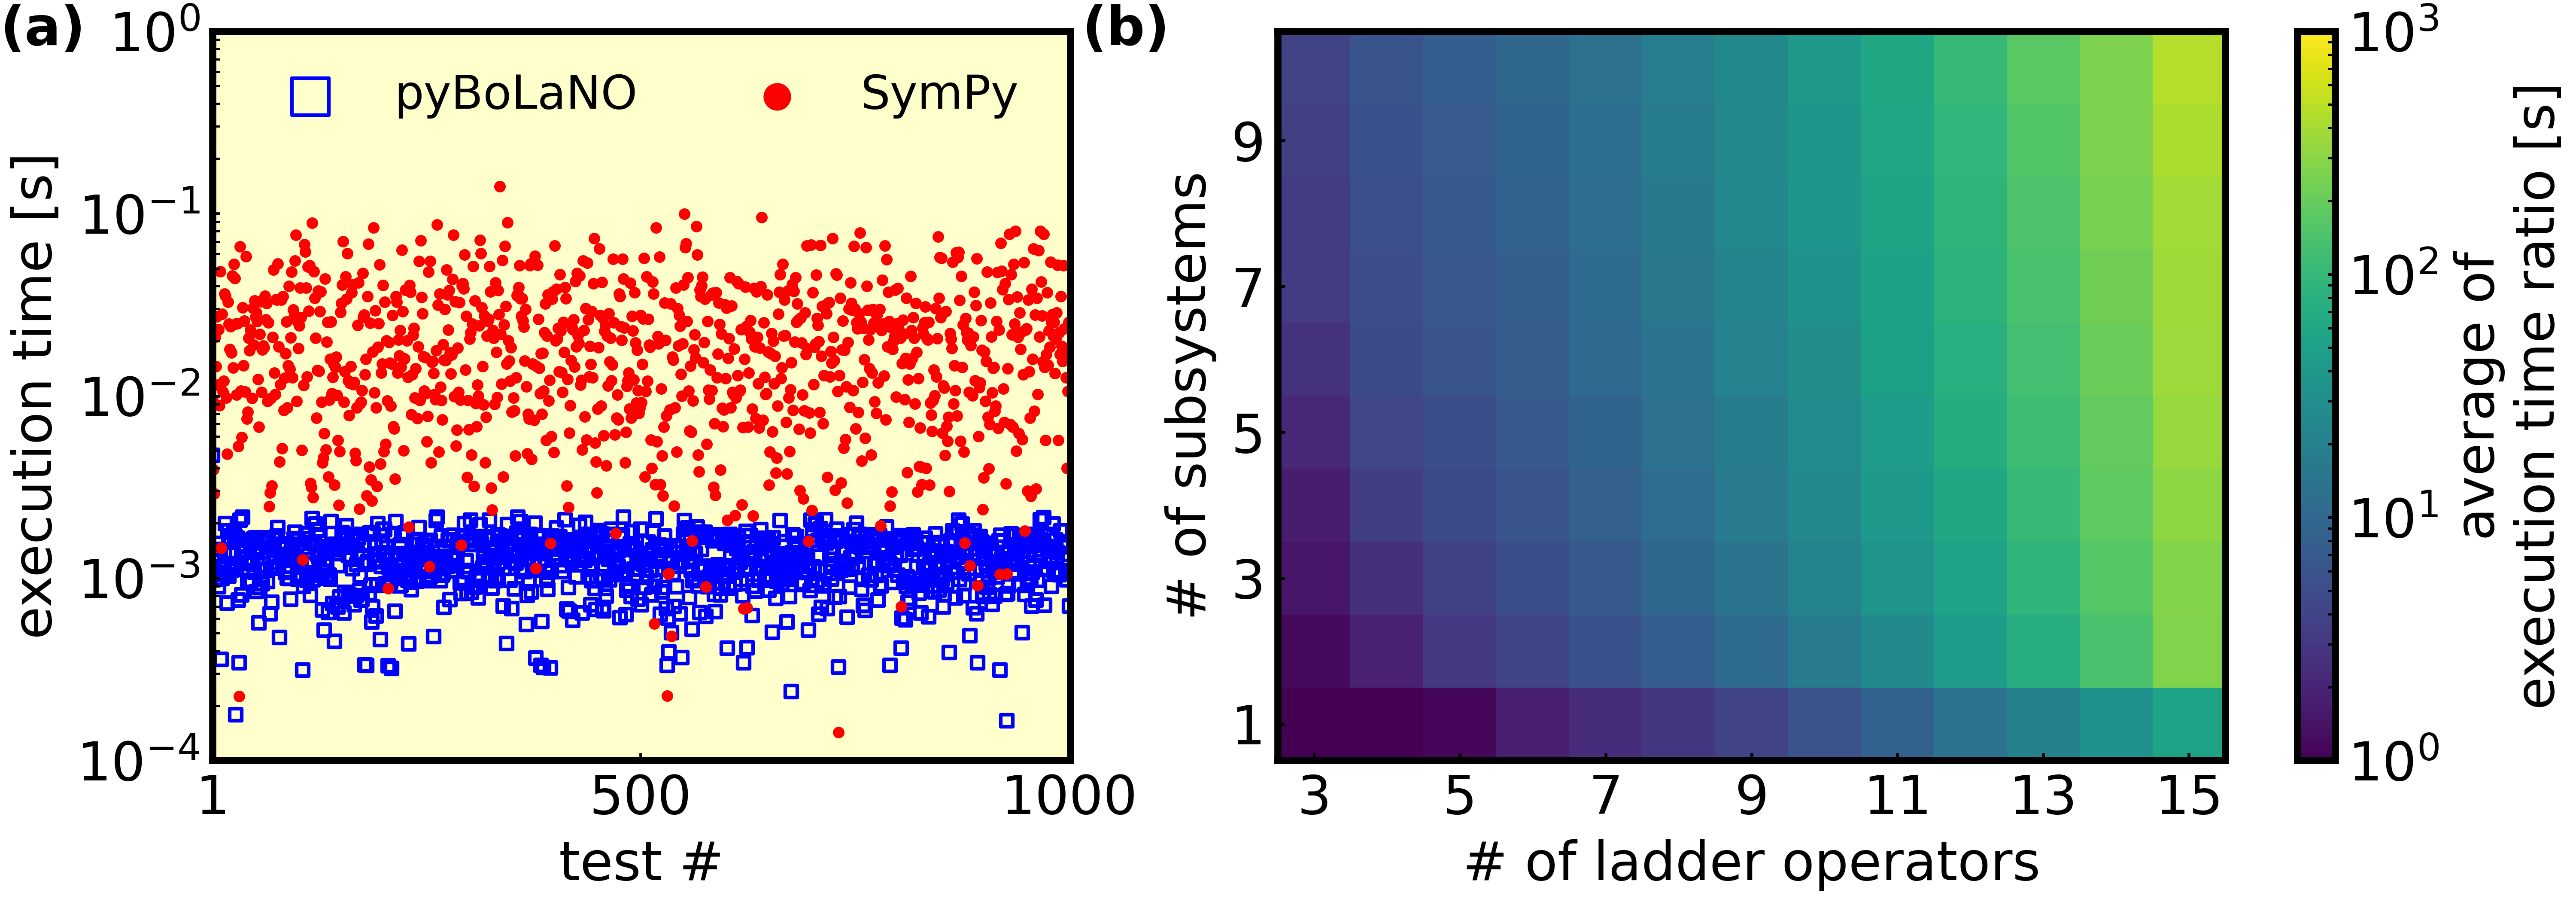
\includegraphics[width=\linewidth]{fig_2.png}
    \caption{\begin{revision}Benchmarks of \texttt{pyBoLaNO}'s normal ordering algorithm against \texttt{sympy.physics.operatorordering.normal\_ordererd\_form} involving random ladder operator monomials. \textbf{Benchmark (a):} execution time of the normal ordering of $1000$ monomials containing $10$ ladder operators of $2$ subsystems. \textbf{Benchmark (b):} Average of the ratio between the average execution time of the normal ordering of $1000$ monomials by \texttt{SymPy} and \texttt{pyBoLaNO}, for varying numbers of ladder operators and subsystems. Note: these results may not be exactly reproducible due to the random nature of the benchmarks.\end{revision}}
    \label{fig_2}
\end{figure}

In our second benchmark, we take the average of the ratio between \texttt{SymPy}'s and our package's execution time over $1000$ random ladder monomials, observing how the value varies with the number of ladder operators in the input and the number of subsystems involved. Figure~\ref{fig_2} (b) shows a log-scale tile plot of our result. Evidently, as the numbers of ladder operators and subsystems increase, \texttt{SymPy}'s average execution time quickly grows to become multiple orders of magnitude above our package. This illustrates the superiority of the explicit formula which we implement.  We finally note that our package's multiprocessing does not help it perform better in these benchmarks since the input is a monomial. \end{revision}

\textbf{(Section 6 of the revised manuscript)}

$\dots$ We have exhibited some examples of use by taking recent results from the literature which also serve to validate the package. We have discussed the computational cost of the normal ordering algorithm, \begin{revision}showing its superiority against the conventional implementation of \texttt{SymPy}.\end{revision} $\dots$

\textbf{(Data Availability)}

$\dots$ The code used for Section 4 is compiled into a \texttt{Jupyter Notebook} available at \href{https://github.com/hendry24/pyBoLaNO/blob/main/tutorial.ipynb}{\seqsplit{https://github.com/hendry24/pyBoLaNO/blob/main/tutorial.ipynb}}. \begin{revision}The code used for Section 5 is compiled into a \texttt{Jupyter Notebook} available at \href{https://github.com/hendry24/pyBoLaNO/blob/main/benchmarks.ipynb}{\seqsplit{https://github.com/hendry24/pyBoLaNO/blob/main/benchmarks.ipynb}}.\end{revision}

\end{revpost}

%%%

\begin{revq}{4}
This work is focused on analytical evaluation, but more often than not one needs to numerically solve for the dynamics of open quantum systems. It would be nice if the authors showed how to take their output and solve the resulting equations of motion numerically to obtain an output, e.g. a plot of expectation values over time for some system. This would give the reader an end-to-end example that they could extend in their own research.
\end{revq}

\begin{reva}

We thank you for the suggestion. While this is an interesting idea, we believe that with the differential equations obtained, running a numerical simulation with them is a \emph{trivial} matter. This is especially true for our targeted audience, who we believe have taken at least one course in numerical methods for differential equations. Arguably, adding a discussion about numerical methods would break the flow of the manuscript, which is focused on symbolic evaluation. 

\end{reva}

%%%

\addendum

Upon further inspection, we have realized that the term ``normal ordering'' is conventionally used to mean rewriting a given ladder monomial into a normal-ordered monomial $\bdagn{p}\bop^q$ containing the same number of creator and annihilator operators, i.e. Wick ordering. Since this does not regard the commutation relations, the resulting expression is not equivalent to the original. This is \emph{not} what we want to do with our package. Instead, our definition of ``normal ordering`` is to rewrite a given ladder monomial into an equivalent normal-ordered polynomial. We have fixed this misunderstanding in our manuscript by revising the abstract, keywords, program summary, Section 1, and Section 2.1. 

\begin{revpre}

\textbf{(Abstract)}

We present \texttt{pyBoLaNO}, a \texttt{Python} symbolic package based on \texttt{SymPy} to quickly normal-order (Wick-order) any polynomial in bosonic ladder operators. $\dots$

\textit{Keywords:}$\quad$ bosonic ladder operators, normal ordering, Wick ordering, commutator, Lindblad master equation


\textbf{(Program Summmary)}

$\dots$

{\em Nature of problem:} Normal (Wick) ordering involving bosonic ladder operators. 

{\em Solution method:} Blasiak's formulae for the normal ordering of an arbitrary monomial in bosonic ladder operators. Symbolic programming is fully provided by \texttt{SymPy}.

\textbf{(Paragraph 2 of Section 1 of the original manuscript)}

As the system description becomes more complex, the algebraic manipulation of the dynamical equations becomes more tedious and prone to errors. As such, a calculator that does the algebra is desirable. The \texttt{SymPy} package~\cite{meurer_sympy_2017} provides a symbolic computation framework in the \texttt{Python} programming language. At the time of writing this work, \texttt{SymPy} is on release \inlinecode{ver. 1.13.3}, which supports the ladder operators via the \inlinecode{sympy.physics.secondquant} submodule. However, the support is limited to arithmetic operations. The function \inlinecode{wicks} for normal (Wick) ordering is not implemented for bosonic ladder operators. In practice, we often desire to evaluate the normal ordering of operators involving bosonic ladder operators. An example of such cases, which motivates us for this work, is the evolution of the expectation values for open quantum systems described by the Lindblad master equation~\cite{schlosshauer_decoherence_2007, breuer_theory_2002}. If analytical expressions are not the concern, several packages are available to solve the problem numerically, e.g., \texttt{QuTiP}~\cite{johansson_qutip_2012, johansson_qutip_2013} and \texttt{QuantumOptics.jl}~\cite{Kramer2018}. Otherwise, to our knowledge~\cite{chia_relaxation_2020, Shen2023, downing_hyperbolic_2024, Krimer2019, Zens2019, Ahmadi2024, Downing2021, Downing2022, Downing2023, BenArosh2021, Amitai2018.PhysRevE.97.052203, Minganti2019, Chimczak2023, Farina2019, Zhang2021}, there is yet a symbolic computational package that facilitates the solution to the problem.

\textbf{(Paragraph 1 of Section 2.1. in the original manuscript)}

Normal ordering (or Wick ordering) means using commutation relations to rewrite the given expression so that all creation operators are written to the left of all annihilation operators.  This is important in quantum field theory to avoid divergent integrals and convenient for calculations via Wick's theorem~\cite{lancaster_quantum_2014}.  In quantum optics, it is convenient for calculations via the optical equivalence theorem~\cite{gerry_introductory_2005}.  The normal ordering of an operator $\hat{A}$ may be denoted by $:\mathrel{\hat{A}}:$, for example,
\setcounter{equation}{14}
\begin{equation}\label{eq:normal_ordering_example}
    :\mathrel{\bop_j\bdag_j\bop_j}: = \bop_j+\bdag_j\bop_j^2
\end{equation}


\end{revpre}

%

\begin{revpost}

\textbf{(Abstract)}

We present \texttt{pyBoLaNO}, a \texttt{Python} symbolic package based on \texttt{SymPy} to quickly normal-order any polynomial in bosonic ladder operators \begin{revision}regarding the canonical commutation relations, using Blasiak's formulae\end{revision}. $\dots$

\textit{Keywords:}$\quad$ bosonic ladder operators, \begin{revision}Blasiak's formulae\end{revision}, normal ordering, commutator, Lindblad master equation

\textbf{(Program Summmary)}

$\dots$

{\em Nature of problem:} Normal ordering involving bosonic ladder operators \begin{revision} regarding the canonical commutation relations. \end{revision}

{\em Solution method:} Blasiak's formulae for the normal ordering of an arbitrary monomial in bosonic ladder operators \begin{revision}regarding the canonical commutation relations.\end{revision} Symbolic programming is fully provided by \texttt{SymPy}.

\textbf{(Paragraph 2--3 of Section 1 of the revised manuscript)}

\begin{revision}We are interested in obtaining the normal-ordered equivalent of a polynomial in the ladder operators---a process we shall call ``normal ordering'' herein. This is useful in quantum optics as physically relevant expectation values involve normal-ordered monomials in the ladder operators. Matrix elements in the coherent-state basis can be straightforwardly evaluated for normal-ordered monomials. Furthermore, given the system's Glauber-Sudarshan $P$ function, the normal-ordered form is convenient via the optical equivalence theorem~\cite{gerry_introductory_2005, fox2006quantum}. It is also quite common in the literature to present the evolution equation for a given expectation value in a normal-ordered form~\cite{chia_relaxation_2020, Shen2023, downing_hyperbolic_2024, Krimer2019, Zens2019, Ahmadi2024, Downing2021, Downing2022, Downing2023, BenArosh2021, Amitai2018.PhysRevE.97.052203, Minganti2019, Chimczak2023, Farina2019, Zhang2021}.\end{revision} As the system description becomes more complex, the algebraic manipulation of the dynamical equations becomes more tedious and prone to errors, making automation desirable.

The \texttt{SymPy} package~\cite{meurer_sympy_2017} provides a symbolic computation framework in the \texttt{Python} programming language. At the time of writing this work, \texttt{SymPy} is on release \inlinecode{ver. 1.13.3} which supports the ladder operators via the \inlinecode{sympy.physics.secondquant} and \inlinecode{sympy.physics.quantum} submodules. In particular, normal ordering is implemented as the function \inlinecode{normal_ordered_form}. Unfortunately, the algorithm implemented in the package quickly slows down as we increase the complexity of the expression to normal-order.

\textbf{(Paragraph 1--2 of Section 2.1. in the revised manuscript)}

\begin{revision}Let us consider a monomial in the ladder operators, such as $\bdag\bop\bdag$ or $\bop^2\bdagn{2}$. A ladder monomial is said to be \emph{normal-ordered} if all creation operators are positioned to the left of all annihilation operators, i.e. a monomial of the form $\bdagn{p}\bop^q; p,q\in\mathbb{Z}$. Conventionally, the term ``normal ordering'' refers to Wick ordering, where a given monomial is replaced with an \emph{inequivalent} normal-ordered monomial containing the same number of creation and annihilation operators. It is represented by the ``double dot enclosure'', e.g. $:\mathrel{\bdag\bop\bdag}:=\bdagn{2}\bop$ and $:\mathrel{\bop^2\bdagn{2}}:=\bdagn{2}\bop^2$. In other words, the monomial has been reordered with $\comm{\bop_j}{\bdag_k}=0$ (instead of $\delta_{jk}$). In quantum field theory, Wick ordering is useful to avoid infinite self-energy and to develop the Wick's theorem (see, for example, Chaps. 4 and 18 in Ref.~\cite{lancaster_quantum_2014}). In quantum optics, it is useful to simplify equations in quadrature squeezing (see, for example, Chapter 7 in Ref.~\cite{gerry_introductory_2005}).

Throughout this paper, we define ``normal ordering'' as rewriting the monomial into an \emph{equivalent} expression using the commutation relations. The normal ordering of a ladder monomial $\hat{X}$ is denoted $\mathcal{N}\left(\hat{X}\right)$ herein, for example,
\setcounter{equation}{14}
\begin{equation}
    \mathcal{N}\left(\bdag\bop\bdag\right) = \bdag+\bdagn{2}\bop
\end{equation}
This is useful in quantum optics when dealing with coherent states of the harmonic oscillator, i.e. the state $\ket{\beta}$ satisfying $\bop\ket{\beta} = \beta\ket{\beta}, \beta\in\mathbb{Z}$, which implies that the matrix element $\matrixel{\beta}{\hat{X}}{\beta}$ of some monomial $\hat{X}$ in the coherent state basis can be straightforwardly evaluated if $\hat{X}$ is normal-ordered. It means if $g_\mathcal{N}\left(\bop,\bdag\right)$ is a normal-ordered polynomial in the ladder operators, then
\begin{equation}
    \matrixel{\beta}{g_\mathcal{N}\left(\bop,\bdag\right)}{\beta} = g_\mathcal{N}\left(\beta,\beta^*\right) .
\end{equation}
One interesting property is the optical equivalence theorem. Let $P(\beta)$ be the Glauber-Sudarshan $P$ function, one of the possible phase-space representations of a quantum system; then,
\begin{equation}\begin{split}
    \expval{g_\mathcal{N}\left(\bop,\bdag\right)} = \int \mathrm{d}^2\beta\ P\left(\beta\right)g_\mathcal{N}\left(\beta,\beta^*\right)
\end{split}\end{equation}
which means that we can conveniently obtain the expectation value of any ladder polynomial by normal-ordering the operator and replacing $\left(\bop,\bdag\right)$ by $\left(\beta,\beta^*\right)$, turning the expectation value integral into a simpler weighted average~\cite[Chapter 3]{gerry_introductory_2005}.
\end{revision}

\end{revpost}

%%%

\newpage
\phantomsection

\bibliographystyle{unsrt}
\bibliography{bibliography}

\end{document}